% Created by tikzDevice version 0.12.3.2 on 2022-02-01 17:56:23
% !TEX encoding = UTF-8 Unicode
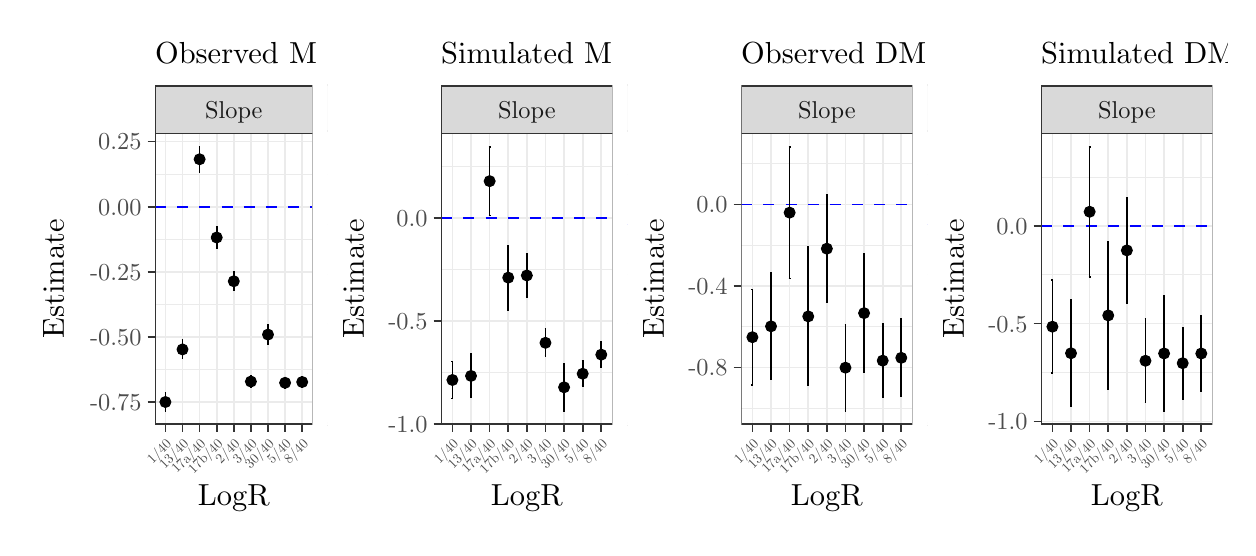
\begin{tikzpicture}[x=1pt,y=1pt]
\definecolor{fillColor}{RGB}{255,255,255}
\path[use as bounding box,fill=fillColor,fill opacity=0.00] (0,0) rectangle (433.62,180.67);
\begin{scope}
\path[clip] (  0.00,  0.00) rectangle (433.62,180.67);
\definecolor{drawColor}{RGB}{255,255,255}
\definecolor{fillColor}{RGB}{255,255,255}

\path[draw=drawColor,line width= 0.6pt,line join=round,line cap=round,fill=fillColor] (  0.00, -0.00) rectangle (433.62,180.67);
\end{scope}
\begin{scope}
\path[clip] ( 37.09, 36.84) rectangle (428.12,143.39);
\definecolor{fillColor}{RGB}{255,255,255}

\path[fill=fillColor] ( 37.09, 36.84) rectangle (428.12,143.39);
\definecolor{drawColor}{gray}{0.92}

\path[draw=drawColor,line width= 0.3pt,line join=round] ( 37.09, 55.79) --
	(428.12, 55.79);

\path[draw=drawColor,line width= 0.3pt,line join=round] ( 37.09, 91.64) --
	(428.12, 91.64);

\path[draw=drawColor,line width= 0.3pt,line join=round] ( 37.09,127.49) --
	(428.12,127.49);

\path[draw=drawColor,line width= 0.6pt,line join=round] ( 37.09, 37.87) --
	(428.12, 37.87);

\path[draw=drawColor,line width= 0.6pt,line join=round] ( 37.09, 73.72) --
	(428.12, 73.72);

\path[draw=drawColor,line width= 0.6pt,line join=round] ( 37.09,109.56) --
	(428.12,109.56);

\path[draw=drawColor,line width= 0.6pt,line join=round] ( 62.59, 36.84) --
	( 62.59,143.39);

\path[draw=drawColor,line width= 0.6pt,line join=round] (105.09, 36.84) --
	(105.09,143.39);

\path[draw=drawColor,line width= 0.6pt,line join=round] (147.60, 36.84) --
	(147.60,143.39);

\path[draw=drawColor,line width= 0.6pt,line join=round] (190.10, 36.84) --
	(190.10,143.39);

\path[draw=drawColor,line width= 0.6pt,line join=round] (232.60, 36.84) --
	(232.60,143.39);

\path[draw=drawColor,line width= 0.6pt,line join=round] (275.11, 36.84) --
	(275.11,143.39);

\path[draw=drawColor,line width= 0.6pt,line join=round] (317.61, 36.84) --
	(317.61,143.39);

\path[draw=drawColor,line width= 0.6pt,line join=round] (360.11, 36.84) --
	(360.11,143.39);

\path[draw=drawColor,line width= 0.6pt,line join=round] (402.62, 36.84) --
	(402.62,143.39);
\definecolor{drawColor}{RGB}{0,0,255}

\path[draw=drawColor,line width= 0.6pt,dash pattern=on 4pt off 4pt ,line join=round] ( 37.09,109.56) -- (428.12,109.56);
\definecolor{drawColor}{RGB}{0,0,0}
\definecolor{fillColor}{RGB}{0,0,0}

\path[draw=drawColor,line width= 0.4pt,line join=round,line cap=round,fill=fillColor] ( 62.59, 72.59) circle (  1.96);

\path[draw=drawColor,line width= 0.4pt,line join=round,line cap=round,fill=fillColor] (232.60,100.56) circle (  1.96);

\path[draw=drawColor,line width= 0.4pt,line join=round,line cap=round,fill=fillColor] (275.11, 60.08) circle (  1.96);

\path[draw=drawColor,line width= 0.4pt,line join=round,line cap=round,fill=fillColor] (360.11, 59.21) circle (  1.96);

\path[draw=drawColor,line width= 0.4pt,line join=round,line cap=round,fill=fillColor] (402.62, 62.76) circle (  1.96);

\path[draw=drawColor,line width= 0.4pt,line join=round,line cap=round,fill=fillColor] (105.09, 62.85) circle (  1.96);

\path[draw=drawColor,line width= 0.4pt,line join=round,line cap=round,fill=fillColor] (147.60,114.72) circle (  1.96);

\path[draw=drawColor,line width= 0.4pt,line join=round,line cap=round,fill=fillColor] (190.10, 76.72) circle (  1.96);

\path[draw=drawColor,line width= 0.4pt,line join=round,line cap=round,fill=fillColor] (317.61, 62.78) circle (  1.96);

\path[draw=drawColor,line width= 0.6pt,line join=round] ( 60.47, 89.64) --
	( 64.72, 89.64);

\path[draw=drawColor,line width= 0.6pt,line join=round] ( 62.59, 89.64) --
	( 62.59, 55.54);

\path[draw=drawColor,line width= 0.6pt,line join=round] ( 60.47, 55.54) --
	( 64.72, 55.54);

\path[draw=drawColor,line width= 0.6pt,line join=round] (230.48,119.92) --
	(234.73,119.92);

\path[draw=drawColor,line width= 0.6pt,line join=round] (232.60,119.92) --
	(232.60, 81.21);

\path[draw=drawColor,line width= 0.6pt,line join=round] (230.48, 81.21) --
	(234.73, 81.21);

\path[draw=drawColor,line width= 0.6pt,line join=round] (272.98, 75.42) --
	(277.23, 75.42);

\path[draw=drawColor,line width= 0.6pt,line join=round] (275.11, 75.42) --
	(275.11, 44.74);

\path[draw=drawColor,line width= 0.6pt,line join=round] (272.98, 44.74) --
	(277.23, 44.74);

\path[draw=drawColor,line width= 0.6pt,line join=round] (357.99, 72.34) --
	(362.24, 72.34);

\path[draw=drawColor,line width= 0.6pt,line join=round] (360.11, 72.34) --
	(360.11, 46.08);

\path[draw=drawColor,line width= 0.6pt,line join=round] (357.99, 46.08) --
	(362.24, 46.08);

\path[draw=drawColor,line width= 0.6pt,line join=round] (400.49, 76.48) --
	(404.74, 76.48);

\path[draw=drawColor,line width= 0.6pt,line join=round] (402.62, 76.48) --
	(402.62, 49.03);

\path[draw=drawColor,line width= 0.6pt,line join=round] (400.49, 49.03) --
	(404.74, 49.03);

\path[draw=drawColor,line width= 0.6pt,line join=round] (102.97, 82.37) --
	(107.22, 82.37);

\path[draw=drawColor,line width= 0.6pt,line join=round] (105.09, 82.37) --
	(105.09, 43.33);

\path[draw=drawColor,line width= 0.6pt,line join=round] (102.97, 43.33) --
	(107.22, 43.33);

\path[draw=drawColor,line width= 0.6pt,line join=round] (145.47,138.55) --
	(149.72,138.55);

\path[draw=drawColor,line width= 0.6pt,line join=round] (147.60,138.55) --
	(147.60, 90.90);

\path[draw=drawColor,line width= 0.6pt,line join=round] (145.47, 90.90) --
	(149.72, 90.90);

\path[draw=drawColor,line width= 0.6pt,line join=round] (187.98,103.79) --
	(192.23,103.79);

\path[draw=drawColor,line width= 0.6pt,line join=round] (190.10,103.79) --
	(190.10, 49.65);

\path[draw=drawColor,line width= 0.6pt,line join=round] (187.98, 49.65) --
	(192.23, 49.65);

\path[draw=drawColor,line width= 0.6pt,line join=round] (315.49, 83.87) --
	(319.74, 83.87);

\path[draw=drawColor,line width= 0.6pt,line join=round] (317.61, 83.87) --
	(317.61, 41.68);

\path[draw=drawColor,line width= 0.6pt,line join=round] (315.49, 41.68) --
	(319.74, 41.68);
\definecolor{drawColor}{gray}{0.20}

\path[draw=drawColor,line width= 0.6pt,line join=round,line cap=round] ( 37.09, 36.84) rectangle (428.12,143.39);
\end{scope}
\begin{scope}
\path[clip] ( 37.09,143.39) rectangle (428.12,159.96);
\definecolor{drawColor}{gray}{0.20}
\definecolor{fillColor}{gray}{0.85}

\path[draw=drawColor,line width= 0.6pt,line join=round,line cap=round,fill=fillColor] ( 37.09,143.39) rectangle (428.12,159.96);
\definecolor{drawColor}{gray}{0.10}

\node[text=drawColor,anchor=base,inner sep=0pt, outer sep=0pt, scale=  0.88] at (232.60,148.64) {Slope};
\end{scope}
\begin{scope}
\path[clip] (  0.00,  0.00) rectangle (433.62,180.67);
\definecolor{drawColor}{gray}{0.20}

\path[draw=drawColor,line width= 0.6pt,line join=round] ( 62.59, 34.09) --
	( 62.59, 36.84);

\path[draw=drawColor,line width= 0.6pt,line join=round] (105.09, 34.09) --
	(105.09, 36.84);

\path[draw=drawColor,line width= 0.6pt,line join=round] (147.60, 34.09) --
	(147.60, 36.84);

\path[draw=drawColor,line width= 0.6pt,line join=round] (190.10, 34.09) --
	(190.10, 36.84);

\path[draw=drawColor,line width= 0.6pt,line join=round] (232.60, 34.09) --
	(232.60, 36.84);

\path[draw=drawColor,line width= 0.6pt,line join=round] (275.11, 34.09) --
	(275.11, 36.84);

\path[draw=drawColor,line width= 0.6pt,line join=round] (317.61, 34.09) --
	(317.61, 36.84);

\path[draw=drawColor,line width= 0.6pt,line join=round] (360.11, 34.09) --
	(360.11, 36.84);

\path[draw=drawColor,line width= 0.6pt,line join=round] (402.62, 34.09) --
	(402.62, 36.84);
\end{scope}
\begin{scope}
\path[clip] (  0.00,  0.00) rectangle (433.62,180.67);
\definecolor{drawColor}{gray}{0.30}

\node[text=drawColor,rotate= 45.00,anchor=base east,inner sep=0pt, outer sep=0pt, scale=  0.50] at ( 65.03, 29.45) {1/40};

\node[text=drawColor,rotate= 45.00,anchor=base east,inner sep=0pt, outer sep=0pt, scale=  0.50] at (107.53, 29.45) {13/40};

\node[text=drawColor,rotate= 45.00,anchor=base east,inner sep=0pt, outer sep=0pt, scale=  0.50] at (150.03, 29.45) {17a/40};

\node[text=drawColor,rotate= 45.00,anchor=base east,inner sep=0pt, outer sep=0pt, scale=  0.50] at (192.54, 29.45) {17b/40};

\node[text=drawColor,rotate= 45.00,anchor=base east,inner sep=0pt, outer sep=0pt, scale=  0.50] at (235.04, 29.45) {2/40};

\node[text=drawColor,rotate= 45.00,anchor=base east,inner sep=0pt, outer sep=0pt, scale=  0.50] at (277.54, 29.45) {3/40};

\node[text=drawColor,rotate= 45.00,anchor=base east,inner sep=0pt, outer sep=0pt, scale=  0.50] at (320.05, 29.45) {30/40};

\node[text=drawColor,rotate= 45.00,anchor=base east,inner sep=0pt, outer sep=0pt, scale=  0.50] at (362.55, 29.45) {5/40};

\node[text=drawColor,rotate= 45.00,anchor=base east,inner sep=0pt, outer sep=0pt, scale=  0.50] at (405.05, 29.45) {8/40};
\end{scope}
\begin{scope}
\path[clip] (  0.00,  0.00) rectangle (433.62,180.67);
\definecolor{drawColor}{gray}{0.30}

\node[text=drawColor,anchor=base east,inner sep=0pt, outer sep=0pt, scale=  0.88] at ( 32.14, 34.84) {-1.0};

\node[text=drawColor,anchor=base east,inner sep=0pt, outer sep=0pt, scale=  0.88] at ( 32.14, 70.69) {-0.5};

\node[text=drawColor,anchor=base east,inner sep=0pt, outer sep=0pt, scale=  0.88] at ( 32.14,106.53) {0.0};
\end{scope}
\begin{scope}
\path[clip] (  0.00,  0.00) rectangle (433.62,180.67);
\definecolor{drawColor}{gray}{0.20}

\path[draw=drawColor,line width= 0.6pt,line join=round] ( 34.34, 37.87) --
	( 37.09, 37.87);

\path[draw=drawColor,line width= 0.6pt,line join=round] ( 34.34, 73.72) --
	( 37.09, 73.72);

\path[draw=drawColor,line width= 0.6pt,line join=round] ( 34.34,109.56) --
	( 37.09,109.56);
\end{scope}
\begin{scope}
\path[clip] (  0.00,  0.00) rectangle (433.62,180.67);
\definecolor{drawColor}{RGB}{0,0,0}

\node[text=drawColor,anchor=base,inner sep=0pt, outer sep=0pt, scale=  1.10] at (232.60,  7.64) {LogR};
\end{scope}
\begin{scope}
\path[clip] (  0.00,  0.00) rectangle (433.62,180.67);
\definecolor{drawColor}{RGB}{0,0,0}

\node[text=drawColor,rotate= 90.00,anchor=base,inner sep=0pt, outer sep=0pt, scale=  1.10] at ( 13.08, 90.11) {Estimate};
\end{scope}
\begin{scope}
\path[clip] (  0.00,  0.00) rectangle (433.62,180.67);
\definecolor{drawColor}{RGB}{0,0,0}

\node[text=drawColor,anchor=base west,inner sep=0pt, outer sep=0pt, scale=  1.10] at ( 37.09,167.60) {Simulated DM};
\end{scope}
\begin{scope}
\path[clip] (  0.00,  0.00) rectangle (108.41,180.67);
\definecolor{drawColor}{RGB}{255,255,255}
\definecolor{fillColor}{RGB}{255,255,255}

\path[draw=drawColor,line width= 0.6pt,line join=round,line cap=round,fill=fillColor] ( -0.00, -0.00) rectangle (108.41,180.67);
\end{scope}
\begin{scope}
\path[clip] ( 46.06, 37.39) rectangle (102.91,142.40);
\definecolor{fillColor}{RGB}{255,255,255}

\path[fill=fillColor] ( 46.06, 37.39) rectangle (102.91,142.40);
\definecolor{drawColor}{gray}{0.92}

\path[draw=drawColor,line width= 0.3pt,line join=round] ( 46.06, 57.15) --
	(102.91, 57.15);

\path[draw=drawColor,line width= 0.3pt,line join=round] ( 46.06, 80.68) --
	(102.91, 80.68);

\path[draw=drawColor,line width= 0.3pt,line join=round] ( 46.06,104.22) --
	(102.91,104.22);

\path[draw=drawColor,line width= 0.3pt,line join=round] ( 46.06,127.75) --
	(102.91,127.75);

\path[draw=drawColor,line width= 0.6pt,line join=round] ( 46.06, 45.38) --
	(102.91, 45.38);

\path[draw=drawColor,line width= 0.6pt,line join=round] ( 46.06, 68.92) --
	(102.91, 68.92);

\path[draw=drawColor,line width= 0.6pt,line join=round] ( 46.06, 92.45) --
	(102.91, 92.45);

\path[draw=drawColor,line width= 0.6pt,line join=round] ( 46.06,115.98) --
	(102.91,115.98);

\path[draw=drawColor,line width= 0.6pt,line join=round] ( 46.06,139.52) --
	(102.91,139.52);

\path[draw=drawColor,line width= 0.6pt,line join=round] ( 49.77, 37.39) --
	( 49.77,142.40);

\path[draw=drawColor,line width= 0.6pt,line join=round] ( 55.95, 37.39) --
	( 55.95,142.40);

\path[draw=drawColor,line width= 0.6pt,line join=round] ( 62.13, 37.39) --
	( 62.13,142.40);

\path[draw=drawColor,line width= 0.6pt,line join=round] ( 68.30, 37.39) --
	( 68.30,142.40);

\path[draw=drawColor,line width= 0.6pt,line join=round] ( 74.48, 37.39) --
	( 74.48,142.40);

\path[draw=drawColor,line width= 0.6pt,line join=round] ( 80.66, 37.39) --
	( 80.66,142.40);

\path[draw=drawColor,line width= 0.6pt,line join=round] ( 86.84, 37.39) --
	( 86.84,142.40);

\path[draw=drawColor,line width= 0.6pt,line join=round] ( 93.02, 37.39) --
	( 93.02,142.40);

\path[draw=drawColor,line width= 0.6pt,line join=round] ( 99.20, 37.39) --
	( 99.20,142.40);
\definecolor{drawColor}{RGB}{0,0,255}

\path[draw=drawColor,line width= 0.6pt,dash pattern=on 4pt off 4pt ,line join=round] ( 46.06,115.98) -- (102.91,115.98);
\definecolor{drawColor}{RGB}{0,0,0}
\definecolor{fillColor}{RGB}{0,0,0}

\path[draw=drawColor,line width= 0.4pt,line join=round,line cap=round,fill=fillColor] ( 49.77, 45.40) circle (  1.96);

\path[draw=drawColor,line width= 0.4pt,line join=round,line cap=round,fill=fillColor] ( 74.48, 89.04) circle (  1.96);

\path[draw=drawColor,line width= 0.4pt,line join=round,line cap=round,fill=fillColor] ( 80.66, 52.80) circle (  1.96);

\path[draw=drawColor,line width= 0.4pt,line join=round,line cap=round,fill=fillColor] ( 93.02, 52.34) circle (  1.96);

\path[draw=drawColor,line width= 0.4pt,line join=round,line cap=round,fill=fillColor] ( 99.20, 52.63) circle (  1.96);

\path[draw=drawColor,line width= 0.4pt,line join=round,line cap=round,fill=fillColor] ( 55.95, 64.40) circle (  1.96);

\path[draw=drawColor,line width= 0.4pt,line join=round,line cap=round,fill=fillColor] ( 62.13,133.12) circle (  1.96);

\path[draw=drawColor,line width= 0.4pt,line join=round,line cap=round,fill=fillColor] ( 68.30,104.85) circle (  1.96);

\path[draw=drawColor,line width= 0.4pt,line join=round,line cap=round,fill=fillColor] ( 86.84, 69.77) circle (  1.96);

\path[draw=drawColor,line width= 0.6pt,line join=round] ( 49.46, 48.63) --
	( 50.08, 48.63);

\path[draw=drawColor,line width= 0.6pt,line join=round] ( 49.77, 48.63) --
	( 49.77, 42.16);

\path[draw=drawColor,line width= 0.6pt,line join=round] ( 49.46, 42.16) --
	( 50.08, 42.16);

\path[draw=drawColor,line width= 0.6pt,line join=round] ( 74.17, 92.45) --
	( 74.79, 92.45);

\path[draw=drawColor,line width= 0.6pt,line join=round] ( 74.48, 92.45) --
	( 74.48, 85.64);

\path[draw=drawColor,line width= 0.6pt,line join=round] ( 74.17, 85.64) --
	( 74.79, 85.64);

\path[draw=drawColor,line width= 0.6pt,line join=round] ( 80.35, 54.79) --
	( 80.97, 54.79);

\path[draw=drawColor,line width= 0.6pt,line join=round] ( 80.66, 54.79) --
	( 80.66, 50.81);

\path[draw=drawColor,line width= 0.6pt,line join=round] ( 80.35, 50.81) --
	( 80.97, 50.81);

\path[draw=drawColor,line width= 0.6pt,line join=round] ( 92.71, 54.26) --
	( 93.33, 54.26);

\path[draw=drawColor,line width= 0.6pt,line join=round] ( 93.02, 54.26) --
	( 93.02, 50.41);

\path[draw=drawColor,line width= 0.6pt,line join=round] ( 92.71, 50.41) --
	( 93.33, 50.41);

\path[draw=drawColor,line width= 0.6pt,line join=round] ( 98.89, 54.62) --
	( 99.51, 54.62);

\path[draw=drawColor,line width= 0.6pt,line join=round] ( 99.20, 54.62) --
	( 99.20, 50.64);

\path[draw=drawColor,line width= 0.6pt,line join=round] ( 98.89, 50.64) --
	( 99.51, 50.64);

\path[draw=drawColor,line width= 0.6pt,line join=round] ( 55.64, 67.73) --
	( 56.26, 67.73);

\path[draw=drawColor,line width= 0.6pt,line join=round] ( 55.95, 67.73) --
	( 55.95, 61.07);

\path[draw=drawColor,line width= 0.6pt,line join=round] ( 55.64, 61.07) --
	( 56.26, 61.07);

\path[draw=drawColor,line width= 0.6pt,line join=round] ( 61.82,137.62) --
	( 62.43,137.62);

\path[draw=drawColor,line width= 0.6pt,line join=round] ( 62.13,137.62) --
	( 62.13,128.62);

\path[draw=drawColor,line width= 0.6pt,line join=round] ( 61.82,128.62) --
	( 62.43,128.62);

\path[draw=drawColor,line width= 0.6pt,line join=round] ( 68.00,108.83) --
	( 68.61,108.83);

\path[draw=drawColor,line width= 0.6pt,line join=round] ( 68.30,108.83) --
	( 68.30,100.86);

\path[draw=drawColor,line width= 0.6pt,line join=round] ( 68.00,100.86) --
	( 68.61,100.86);

\path[draw=drawColor,line width= 0.6pt,line join=round] ( 86.53, 73.24) --
	( 87.15, 73.24);

\path[draw=drawColor,line width= 0.6pt,line join=round] ( 86.84, 73.24) --
	( 86.84, 66.29);

\path[draw=drawColor,line width= 0.6pt,line join=round] ( 86.53, 66.29) --
	( 87.15, 66.29);
\definecolor{drawColor}{gray}{0.20}

\path[draw=drawColor,line width= 0.6pt,line join=round,line cap=round] ( 46.06, 37.39) rectangle (102.91,142.40);
\end{scope}
\begin{scope}
\path[clip] ( 46.06,142.40) rectangle (102.91,159.67);
\definecolor{drawColor}{gray}{0.20}
\definecolor{fillColor}{gray}{0.85}

\path[draw=drawColor,line width= 0.6pt,line join=round,line cap=round,fill=fillColor] ( 46.06,142.40) rectangle (102.91,159.67);
\definecolor{drawColor}{gray}{0.10}

\node[text=drawColor,anchor=base,inner sep=0pt, outer sep=0pt, scale=  0.88] at ( 74.48,148.00) {Slope};
\end{scope}
\begin{scope}
\path[clip] (  0.00,  0.00) rectangle (433.62,180.67);
\definecolor{drawColor}{gray}{0.20}

\path[draw=drawColor,line width= 0.6pt,line join=round] ( 49.77, 34.64) --
	( 49.77, 37.39);

\path[draw=drawColor,line width= 0.6pt,line join=round] ( 55.95, 34.64) --
	( 55.95, 37.39);

\path[draw=drawColor,line width= 0.6pt,line join=round] ( 62.13, 34.64) --
	( 62.13, 37.39);

\path[draw=drawColor,line width= 0.6pt,line join=round] ( 68.30, 34.64) --
	( 68.30, 37.39);

\path[draw=drawColor,line width= 0.6pt,line join=round] ( 74.48, 34.64) --
	( 74.48, 37.39);

\path[draw=drawColor,line width= 0.6pt,line join=round] ( 80.66, 34.64) --
	( 80.66, 37.39);

\path[draw=drawColor,line width= 0.6pt,line join=round] ( 86.84, 34.64) --
	( 86.84, 37.39);

\path[draw=drawColor,line width= 0.6pt,line join=round] ( 93.02, 34.64) --
	( 93.02, 37.39);

\path[draw=drawColor,line width= 0.6pt,line join=round] ( 99.20, 34.64) --
	( 99.20, 37.39);
\end{scope}
\begin{scope}
\path[clip] (  0.00,  0.00) rectangle (433.62,180.67);
\definecolor{drawColor}{gray}{0.30}

\node[text=drawColor,rotate= 45.00,anchor=base east,inner sep=0pt, outer sep=0pt, scale=  0.50] at ( 52.20, 30.00) {1/40};

\node[text=drawColor,rotate= 45.00,anchor=base east,inner sep=0pt, outer sep=0pt, scale=  0.50] at ( 58.38, 30.00) {13/40};

\node[text=drawColor,rotate= 45.00,anchor=base east,inner sep=0pt, outer sep=0pt, scale=  0.50] at ( 64.56, 30.00) {17a/40};

\node[text=drawColor,rotate= 45.00,anchor=base east,inner sep=0pt, outer sep=0pt, scale=  0.50] at ( 70.74, 30.00) {17b/40};

\node[text=drawColor,rotate= 45.00,anchor=base east,inner sep=0pt, outer sep=0pt, scale=  0.50] at ( 76.92, 30.00) {2/40};

\node[text=drawColor,rotate= 45.00,anchor=base east,inner sep=0pt, outer sep=0pt, scale=  0.50] at ( 83.10, 30.00) {3/40};

\node[text=drawColor,rotate= 45.00,anchor=base east,inner sep=0pt, outer sep=0pt, scale=  0.50] at ( 89.28, 30.00) {30/40};

\node[text=drawColor,rotate= 45.00,anchor=base east,inner sep=0pt, outer sep=0pt, scale=  0.50] at ( 95.45, 30.00) {5/40};

\node[text=drawColor,rotate= 45.00,anchor=base east,inner sep=0pt, outer sep=0pt, scale=  0.50] at (101.63, 30.00) {8/40};
\end{scope}
\begin{scope}
\path[clip] (  0.00,  0.00) rectangle (433.62,180.67);
\definecolor{drawColor}{gray}{0.30}

\node[text=drawColor,anchor=base east,inner sep=0pt, outer sep=0pt, scale=  0.88] at ( 41.11, 42.35) {-0.75};

\node[text=drawColor,anchor=base east,inner sep=0pt, outer sep=0pt, scale=  0.88] at ( 41.11, 65.89) {-0.50};

\node[text=drawColor,anchor=base east,inner sep=0pt, outer sep=0pt, scale=  0.88] at ( 41.11, 89.42) {-0.25};

\node[text=drawColor,anchor=base east,inner sep=0pt, outer sep=0pt, scale=  0.88] at ( 41.11,112.95) {0.00};

\node[text=drawColor,anchor=base east,inner sep=0pt, outer sep=0pt, scale=  0.88] at ( 41.11,136.49) {0.25};
\end{scope}
\begin{scope}
\path[clip] (  0.00,  0.00) rectangle (433.62,180.67);
\definecolor{drawColor}{gray}{0.20}

\path[draw=drawColor,line width= 0.6pt,line join=round] ( 43.31, 45.38) --
	( 46.06, 45.38);

\path[draw=drawColor,line width= 0.6pt,line join=round] ( 43.31, 68.92) --
	( 46.06, 68.92);

\path[draw=drawColor,line width= 0.6pt,line join=round] ( 43.31, 92.45) --
	( 46.06, 92.45);

\path[draw=drawColor,line width= 0.6pt,line join=round] ( 43.31,115.98) --
	( 46.06,115.98);

\path[draw=drawColor,line width= 0.6pt,line join=round] ( 43.31,139.52) --
	( 46.06,139.52);
\end{scope}
\begin{scope}
\path[clip] (  0.00,  0.00) rectangle (433.62,180.67);
\definecolor{drawColor}{RGB}{0,0,0}

\node[text=drawColor,anchor=base,inner sep=0pt, outer sep=0pt, scale=  1.10] at ( 74.48,  7.93) {LogR};
\end{scope}
\begin{scope}
\path[clip] (  0.00,  0.00) rectangle (433.62,180.67);
\definecolor{drawColor}{RGB}{0,0,0}

\node[text=drawColor,rotate= 90.00,anchor=base,inner sep=0pt, outer sep=0pt, scale=  1.10] at ( 13.08, 89.89) {Estimate};
\end{scope}
\begin{scope}
\path[clip] (  0.00,  0.00) rectangle (433.62,180.67);
\definecolor{drawColor}{RGB}{0,0,0}

\node[text=drawColor,anchor=base west,inner sep=0pt, outer sep=0pt, scale=  1.10] at ( 46.06,167.60) {Observed M};
\end{scope}
\begin{scope}
\path[clip] (108.41,  0.00) rectangle (216.81,180.67);
\definecolor{drawColor}{RGB}{255,255,255}
\definecolor{fillColor}{RGB}{255,255,255}

\path[draw=drawColor,line width= 0.6pt,line join=round,line cap=round,fill=fillColor] (108.41, -0.00) rectangle (216.81,180.67);
\end{scope}
\begin{scope}
\path[clip] (149.44, 37.39) rectangle (211.31,142.40);
\definecolor{fillColor}{RGB}{255,255,255}

\path[fill=fillColor] (149.44, 37.39) rectangle (211.31,142.40);
\definecolor{drawColor}{gray}{0.92}

\path[draw=drawColor,line width= 0.3pt,line join=round] (149.44, 56.07) --
	(211.31, 56.07);

\path[draw=drawColor,line width= 0.3pt,line join=round] (149.44, 93.32) --
	(211.31, 93.32);

\path[draw=drawColor,line width= 0.3pt,line join=round] (149.44,130.56) --
	(211.31,130.56);

\path[draw=drawColor,line width= 0.6pt,line join=round] (149.44, 37.45) --
	(211.31, 37.45);

\path[draw=drawColor,line width= 0.6pt,line join=round] (149.44, 74.69) --
	(211.31, 74.69);

\path[draw=drawColor,line width= 0.6pt,line join=round] (149.44,111.94) --
	(211.31,111.94);

\path[draw=drawColor,line width= 0.6pt,line join=round] (153.48, 37.39) --
	(153.48,142.40);

\path[draw=drawColor,line width= 0.6pt,line join=round] (160.20, 37.39) --
	(160.20,142.40);

\path[draw=drawColor,line width= 0.6pt,line join=round] (166.93, 37.39) --
	(166.93,142.40);

\path[draw=drawColor,line width= 0.6pt,line join=round] (173.65, 37.39) --
	(173.65,142.40);

\path[draw=drawColor,line width= 0.6pt,line join=round] (180.38, 37.39) --
	(180.38,142.40);

\path[draw=drawColor,line width= 0.6pt,line join=round] (187.10, 37.39) --
	(187.10,142.40);

\path[draw=drawColor,line width= 0.6pt,line join=round] (193.83, 37.39) --
	(193.83,142.40);

\path[draw=drawColor,line width= 0.6pt,line join=round] (200.55, 37.39) --
	(200.55,142.40);

\path[draw=drawColor,line width= 0.6pt,line join=round] (207.28, 37.39) --
	(207.28,142.40);
\definecolor{drawColor}{RGB}{0,0,255}

\path[draw=drawColor,line width= 0.6pt,dash pattern=on 4pt off 4pt ,line join=round] (149.44,111.94) -- (211.31,111.94);
\definecolor{drawColor}{RGB}{0,0,0}
\definecolor{fillColor}{RGB}{0,0,0}

\path[draw=drawColor,line width= 0.4pt,line join=round,line cap=round,fill=fillColor] (153.48, 53.36) circle (  1.96);

\path[draw=drawColor,line width= 0.4pt,line join=round,line cap=round,fill=fillColor] (180.38, 91.13) circle (  1.96);

\path[draw=drawColor,line width= 0.4pt,line join=round,line cap=round,fill=fillColor] (187.10, 66.79) circle (  1.96);

\path[draw=drawColor,line width= 0.4pt,line join=round,line cap=round,fill=fillColor] (200.55, 55.62) circle (  1.96);

\path[draw=drawColor,line width= 0.4pt,line join=round,line cap=round,fill=fillColor] (207.28, 62.52) circle (  1.96);

\path[draw=drawColor,line width= 0.4pt,line join=round,line cap=round,fill=fillColor] (160.20, 54.83) circle (  1.96);

\path[draw=drawColor,line width= 0.4pt,line join=round,line cap=round,fill=fillColor] (166.93,125.21) circle (  1.96);

\path[draw=drawColor,line width= 0.4pt,line join=round,line cap=round,fill=fillColor] (173.65, 90.35) circle (  1.96);

\path[draw=drawColor,line width= 0.4pt,line join=round,line cap=round,fill=fillColor] (193.83, 50.72) circle (  1.96);

\path[draw=drawColor,line width= 0.6pt,line join=round] (153.14, 60.03) --
	(153.81, 60.03);

\path[draw=drawColor,line width= 0.6pt,line join=round] (153.48, 60.03) --
	(153.48, 46.69);

\path[draw=drawColor,line width= 0.6pt,line join=round] (153.14, 46.69) --
	(153.81, 46.69);

\path[draw=drawColor,line width= 0.6pt,line join=round] (180.04, 99.04) --
	(180.71, 99.04);

\path[draw=drawColor,line width= 0.6pt,line join=round] (180.38, 99.04) --
	(180.38, 83.23);

\path[draw=drawColor,line width= 0.6pt,line join=round] (180.04, 83.23) --
	(180.71, 83.23);

\path[draw=drawColor,line width= 0.6pt,line join=round] (186.76, 71.67) --
	(187.44, 71.67);

\path[draw=drawColor,line width= 0.6pt,line join=round] (187.10, 71.67) --
	(187.10, 61.92);

\path[draw=drawColor,line width= 0.6pt,line join=round] (186.76, 61.92) --
	(187.44, 61.92);

\path[draw=drawColor,line width= 0.6pt,line join=round] (200.21, 60.12) --
	(200.89, 60.12);

\path[draw=drawColor,line width= 0.6pt,line join=round] (200.55, 60.12) --
	(200.55, 51.11);

\path[draw=drawColor,line width= 0.6pt,line join=round] (200.21, 51.11) --
	(200.89, 51.11);

\path[draw=drawColor,line width= 0.6pt,line join=round] (206.94, 67.15) --
	(207.61, 67.15);

\path[draw=drawColor,line width= 0.6pt,line join=round] (207.28, 67.15) --
	(207.28, 57.89);

\path[draw=drawColor,line width= 0.6pt,line join=round] (206.94, 57.89) --
	(207.61, 57.89);

\path[draw=drawColor,line width= 0.6pt,line join=round] (159.87, 62.69) --
	(160.54, 62.69);

\path[draw=drawColor,line width= 0.6pt,line join=round] (160.20, 62.69) --
	(160.20, 46.98);

\path[draw=drawColor,line width= 0.6pt,line join=round] (159.87, 46.98) --
	(160.54, 46.98);

\path[draw=drawColor,line width= 0.6pt,line join=round] (166.59,137.62) --
	(167.26,137.62);

\path[draw=drawColor,line width= 0.6pt,line join=round] (166.93,137.62) --
	(166.93,112.79);

\path[draw=drawColor,line width= 0.6pt,line join=round] (166.59,112.79) --
	(167.26,112.79);

\path[draw=drawColor,line width= 0.6pt,line join=round] (173.32,102.01) --
	(173.99,102.01);

\path[draw=drawColor,line width= 0.6pt,line join=round] (173.65,102.01) --
	(173.65, 78.69);

\path[draw=drawColor,line width= 0.6pt,line join=round] (173.32, 78.69) --
	(173.99, 78.69);

\path[draw=drawColor,line width= 0.6pt,line join=round] (193.49, 59.28) --
	(194.16, 59.28);

\path[draw=drawColor,line width= 0.6pt,line join=round] (193.83, 59.28) --
	(193.83, 42.16);

\path[draw=drawColor,line width= 0.6pt,line join=round] (193.49, 42.16) --
	(194.16, 42.16);
\definecolor{drawColor}{gray}{0.20}

\path[draw=drawColor,line width= 0.6pt,line join=round,line cap=round] (149.44, 37.39) rectangle (211.31,142.40);
\end{scope}
\begin{scope}
\path[clip] (149.44,142.40) rectangle (211.31,159.67);
\definecolor{drawColor}{gray}{0.20}
\definecolor{fillColor}{gray}{0.85}

\path[draw=drawColor,line width= 0.6pt,line join=round,line cap=round,fill=fillColor] (149.44,142.40) rectangle (211.31,159.67);
\definecolor{drawColor}{gray}{0.10}

\node[text=drawColor,anchor=base,inner sep=0pt, outer sep=0pt, scale=  0.88] at (180.38,148.00) {Slope};
\end{scope}
\begin{scope}
\path[clip] (  0.00,  0.00) rectangle (433.62,180.67);
\definecolor{drawColor}{gray}{0.20}

\path[draw=drawColor,line width= 0.6pt,line join=round] (153.48, 34.64) --
	(153.48, 37.39);

\path[draw=drawColor,line width= 0.6pt,line join=round] (160.20, 34.64) --
	(160.20, 37.39);

\path[draw=drawColor,line width= 0.6pt,line join=round] (166.93, 34.64) --
	(166.93, 37.39);

\path[draw=drawColor,line width= 0.6pt,line join=round] (173.65, 34.64) --
	(173.65, 37.39);

\path[draw=drawColor,line width= 0.6pt,line join=round] (180.38, 34.64) --
	(180.38, 37.39);

\path[draw=drawColor,line width= 0.6pt,line join=round] (187.10, 34.64) --
	(187.10, 37.39);

\path[draw=drawColor,line width= 0.6pt,line join=round] (193.83, 34.64) --
	(193.83, 37.39);

\path[draw=drawColor,line width= 0.6pt,line join=round] (200.55, 34.64) --
	(200.55, 37.39);

\path[draw=drawColor,line width= 0.6pt,line join=round] (207.28, 34.64) --
	(207.28, 37.39);
\end{scope}
\begin{scope}
\path[clip] (  0.00,  0.00) rectangle (433.62,180.67);
\definecolor{drawColor}{gray}{0.30}

\node[text=drawColor,rotate= 45.00,anchor=base east,inner sep=0pt, outer sep=0pt, scale=  0.50] at (155.91, 30.00) {1/40};

\node[text=drawColor,rotate= 45.00,anchor=base east,inner sep=0pt, outer sep=0pt, scale=  0.50] at (162.64, 30.00) {13/40};

\node[text=drawColor,rotate= 45.00,anchor=base east,inner sep=0pt, outer sep=0pt, scale=  0.50] at (169.36, 30.00) {17a/40};

\node[text=drawColor,rotate= 45.00,anchor=base east,inner sep=0pt, outer sep=0pt, scale=  0.50] at (176.09, 30.00) {17b/40};

\node[text=drawColor,rotate= 45.00,anchor=base east,inner sep=0pt, outer sep=0pt, scale=  0.50] at (182.81, 30.00) {2/40};

\node[text=drawColor,rotate= 45.00,anchor=base east,inner sep=0pt, outer sep=0pt, scale=  0.50] at (189.54, 30.00) {3/40};

\node[text=drawColor,rotate= 45.00,anchor=base east,inner sep=0pt, outer sep=0pt, scale=  0.50] at (196.26, 30.00) {30/40};

\node[text=drawColor,rotate= 45.00,anchor=base east,inner sep=0pt, outer sep=0pt, scale=  0.50] at (202.99, 30.00) {5/40};

\node[text=drawColor,rotate= 45.00,anchor=base east,inner sep=0pt, outer sep=0pt, scale=  0.50] at (209.71, 30.00) {8/40};
\end{scope}
\begin{scope}
\path[clip] (  0.00,  0.00) rectangle (433.62,180.67);
\definecolor{drawColor}{gray}{0.30}

\node[text=drawColor,anchor=base east,inner sep=0pt, outer sep=0pt, scale=  0.88] at (144.49, 34.42) {-1.0};

\node[text=drawColor,anchor=base east,inner sep=0pt, outer sep=0pt, scale=  0.88] at (144.49, 71.66) {-0.5};

\node[text=drawColor,anchor=base east,inner sep=0pt, outer sep=0pt, scale=  0.88] at (144.49,108.91) {0.0};
\end{scope}
\begin{scope}
\path[clip] (  0.00,  0.00) rectangle (433.62,180.67);
\definecolor{drawColor}{gray}{0.20}

\path[draw=drawColor,line width= 0.6pt,line join=round] (146.69, 37.45) --
	(149.44, 37.45);

\path[draw=drawColor,line width= 0.6pt,line join=round] (146.69, 74.69) --
	(149.44, 74.69);

\path[draw=drawColor,line width= 0.6pt,line join=round] (146.69,111.94) --
	(149.44,111.94);
\end{scope}
\begin{scope}
\path[clip] (  0.00,  0.00) rectangle (433.62,180.67);
\definecolor{drawColor}{RGB}{0,0,0}

\node[text=drawColor,anchor=base,inner sep=0pt, outer sep=0pt, scale=  1.10] at (180.38,  7.93) {LogR};
\end{scope}
\begin{scope}
\path[clip] (  0.00,  0.00) rectangle (433.62,180.67);
\definecolor{drawColor}{RGB}{0,0,0}

\node[text=drawColor,rotate= 90.00,anchor=base,inner sep=0pt, outer sep=0pt, scale=  1.10] at (121.48, 89.89) {Estimate};
\end{scope}
\begin{scope}
\path[clip] (  0.00,  0.00) rectangle (433.62,180.67);
\definecolor{drawColor}{RGB}{0,0,0}

\node[text=drawColor,anchor=base west,inner sep=0pt, outer sep=0pt, scale=  1.10] at (149.44,167.60) {Simulated M};
\end{scope}
\begin{scope}
\path[clip] (216.81,  0.00) rectangle (325.21,180.67);
\definecolor{drawColor}{RGB}{255,255,255}
\definecolor{fillColor}{RGB}{255,255,255}

\path[draw=drawColor,line width= 0.6pt,line join=round,line cap=round,fill=fillColor] (216.81, -0.00) rectangle (325.22,180.67);
\end{scope}
\begin{scope}
\path[clip] (257.85, 37.39) rectangle (319.71,142.40);
\definecolor{fillColor}{RGB}{255,255,255}

\path[fill=fillColor] (257.85, 37.39) rectangle (319.71,142.40);
\definecolor{drawColor}{gray}{0.92}

\path[draw=drawColor,line width= 0.3pt,line join=round] (257.85, 43.14) --
	(319.71, 43.14);

\path[draw=drawColor,line width= 0.3pt,line join=round] (257.85, 72.58) --
	(319.71, 72.58);

\path[draw=drawColor,line width= 0.3pt,line join=round] (257.85,102.02) --
	(319.71,102.02);

\path[draw=drawColor,line width= 0.3pt,line join=round] (257.85,131.46) --
	(319.71,131.46);

\path[draw=drawColor,line width= 0.6pt,line join=round] (257.85, 57.86) --
	(319.71, 57.86);

\path[draw=drawColor,line width= 0.6pt,line join=round] (257.85, 87.30) --
	(319.71, 87.30);

\path[draw=drawColor,line width= 0.6pt,line join=round] (257.85,116.74) --
	(319.71,116.74);

\path[draw=drawColor,line width= 0.6pt,line join=round] (261.88, 37.39) --
	(261.88,142.40);

\path[draw=drawColor,line width= 0.6pt,line join=round] (268.61, 37.39) --
	(268.61,142.40);

\path[draw=drawColor,line width= 0.6pt,line join=round] (275.33, 37.39) --
	(275.33,142.40);

\path[draw=drawColor,line width= 0.6pt,line join=round] (282.06, 37.39) --
	(282.06,142.40);

\path[draw=drawColor,line width= 0.6pt,line join=round] (288.78, 37.39) --
	(288.78,142.40);

\path[draw=drawColor,line width= 0.6pt,line join=round] (295.51, 37.39) --
	(295.51,142.40);

\path[draw=drawColor,line width= 0.6pt,line join=round] (302.23, 37.39) --
	(302.23,142.40);

\path[draw=drawColor,line width= 0.6pt,line join=round] (308.96, 37.39) --
	(308.96,142.40);

\path[draw=drawColor,line width= 0.6pt,line join=round] (315.68, 37.39) --
	(315.68,142.40);
\definecolor{drawColor}{RGB}{0,0,255}

\path[draw=drawColor,line width= 0.6pt,dash pattern=on 4pt off 4pt ,line join=round] (257.85,116.74) -- (319.71,116.74);
\definecolor{drawColor}{RGB}{0,0,0}
\definecolor{fillColor}{RGB}{0,0,0}

\path[draw=drawColor,line width= 0.4pt,line join=round,line cap=round,fill=fillColor] (261.88, 68.82) circle (  1.96);

\path[draw=drawColor,line width= 0.4pt,line join=round,line cap=round,fill=fillColor] (288.78,100.81) circle (  1.96);

\path[draw=drawColor,line width= 0.4pt,line join=round,line cap=round,fill=fillColor] (295.51, 57.81) circle (  1.96);

\path[draw=drawColor,line width= 0.4pt,line join=round,line cap=round,fill=fillColor] (308.96, 60.35) circle (  1.96);

\path[draw=drawColor,line width= 0.4pt,line join=round,line cap=round,fill=fillColor] (315.68, 61.37) circle (  1.96);

\path[draw=drawColor,line width= 0.4pt,line join=round,line cap=round,fill=fillColor] (268.61, 72.75) circle (  1.96);

\path[draw=drawColor,line width= 0.4pt,line join=round,line cap=round,fill=fillColor] (275.33,113.83) circle (  1.96);

\path[draw=drawColor,line width= 0.4pt,line join=round,line cap=round,fill=fillColor] (282.06, 76.34) circle (  1.96);

\path[draw=drawColor,line width= 0.4pt,line join=round,line cap=round,fill=fillColor] (302.23, 77.52) circle (  1.96);

\path[draw=drawColor,line width= 0.6pt,line join=round] (261.55, 86.09) --
	(262.22, 86.09);

\path[draw=drawColor,line width= 0.6pt,line join=round] (261.88, 86.09) --
	(261.88, 51.55);

\path[draw=drawColor,line width= 0.6pt,line join=round] (261.55, 51.55) --
	(262.22, 51.55);

\path[draw=drawColor,line width= 0.6pt,line join=round] (288.45,120.27) --
	(289.12,120.27);

\path[draw=drawColor,line width= 0.6pt,line join=round] (288.78,120.27) --
	(288.78, 81.35);

\path[draw=drawColor,line width= 0.6pt,line join=round] (288.45, 81.35) --
	(289.12, 81.35);

\path[draw=drawColor,line width= 0.6pt,line join=round] (295.17, 73.46) --
	(295.84, 73.46);

\path[draw=drawColor,line width= 0.6pt,line join=round] (295.51, 73.46) --
	(295.51, 42.16);

\path[draw=drawColor,line width= 0.6pt,line join=round] (295.17, 42.16) --
	(295.84, 42.16);

\path[draw=drawColor,line width= 0.6pt,line join=round] (308.62, 73.55) --
	(309.29, 73.55);

\path[draw=drawColor,line width= 0.6pt,line join=round] (308.96, 73.55) --
	(308.96, 47.15);

\path[draw=drawColor,line width= 0.6pt,line join=round] (308.62, 47.15) --
	(309.29, 47.15);

\path[draw=drawColor,line width= 0.6pt,line join=round] (315.34, 75.30) --
	(316.02, 75.30);

\path[draw=drawColor,line width= 0.6pt,line join=round] (315.68, 75.30) --
	(315.68, 47.44);

\path[draw=drawColor,line width= 0.6pt,line join=round] (315.34, 47.44) --
	(316.02, 47.44);

\path[draw=drawColor,line width= 0.6pt,line join=round] (268.27, 91.94) --
	(268.94, 91.94);

\path[draw=drawColor,line width= 0.6pt,line join=round] (268.61, 91.94) --
	(268.61, 53.56);

\path[draw=drawColor,line width= 0.6pt,line join=round] (268.27, 53.56) --
	(268.94, 53.56);

\path[draw=drawColor,line width= 0.6pt,line join=round] (275.00,137.62) --
	(275.67,137.62);

\path[draw=drawColor,line width= 0.6pt,line join=round] (275.33,137.62) --
	(275.33, 90.03);

\path[draw=drawColor,line width= 0.6pt,line join=round] (275.00, 90.03) --
	(275.67, 90.03);

\path[draw=drawColor,line width= 0.6pt,line join=round] (281.72,101.34) --
	(282.39,101.34);

\path[draw=drawColor,line width= 0.6pt,line join=round] (282.06,101.34) --
	(282.06, 51.34);

\path[draw=drawColor,line width= 0.6pt,line join=round] (281.72, 51.34) --
	(282.39, 51.34);

\path[draw=drawColor,line width= 0.6pt,line join=round] (301.89, 98.79) --
	(302.57, 98.79);

\path[draw=drawColor,line width= 0.6pt,line join=round] (302.23, 98.79) --
	(302.23, 56.25);

\path[draw=drawColor,line width= 0.6pt,line join=round] (301.89, 56.25) --
	(302.57, 56.25);
\definecolor{drawColor}{gray}{0.20}

\path[draw=drawColor,line width= 0.6pt,line join=round,line cap=round] (257.85, 37.39) rectangle (319.71,142.40);
\end{scope}
\begin{scope}
\path[clip] (257.85,142.40) rectangle (319.71,159.67);
\definecolor{drawColor}{gray}{0.20}
\definecolor{fillColor}{gray}{0.85}

\path[draw=drawColor,line width= 0.6pt,line join=round,line cap=round,fill=fillColor] (257.85,142.40) rectangle (319.71,159.67);
\definecolor{drawColor}{gray}{0.10}

\node[text=drawColor,anchor=base,inner sep=0pt, outer sep=0pt, scale=  0.88] at (288.78,148.00) {Slope};
\end{scope}
\begin{scope}
\path[clip] (  0.00,  0.00) rectangle (433.62,180.67);
\definecolor{drawColor}{gray}{0.20}

\path[draw=drawColor,line width= 0.6pt,line join=round] (261.88, 34.64) --
	(261.88, 37.39);

\path[draw=drawColor,line width= 0.6pt,line join=round] (268.61, 34.64) --
	(268.61, 37.39);

\path[draw=drawColor,line width= 0.6pt,line join=round] (275.33, 34.64) --
	(275.33, 37.39);

\path[draw=drawColor,line width= 0.6pt,line join=round] (282.06, 34.64) --
	(282.06, 37.39);

\path[draw=drawColor,line width= 0.6pt,line join=round] (288.78, 34.64) --
	(288.78, 37.39);

\path[draw=drawColor,line width= 0.6pt,line join=round] (295.51, 34.64) --
	(295.51, 37.39);

\path[draw=drawColor,line width= 0.6pt,line join=round] (302.23, 34.64) --
	(302.23, 37.39);

\path[draw=drawColor,line width= 0.6pt,line join=round] (308.96, 34.64) --
	(308.96, 37.39);

\path[draw=drawColor,line width= 0.6pt,line join=round] (315.68, 34.64) --
	(315.68, 37.39);
\end{scope}
\begin{scope}
\path[clip] (  0.00,  0.00) rectangle (433.62,180.67);
\definecolor{drawColor}{gray}{0.30}

\node[text=drawColor,rotate= 45.00,anchor=base east,inner sep=0pt, outer sep=0pt, scale=  0.50] at (264.32, 30.00) {1/40};

\node[text=drawColor,rotate= 45.00,anchor=base east,inner sep=0pt, outer sep=0pt, scale=  0.50] at (271.04, 30.00) {13/40};

\node[text=drawColor,rotate= 45.00,anchor=base east,inner sep=0pt, outer sep=0pt, scale=  0.50] at (277.77, 30.00) {17a/40};

\node[text=drawColor,rotate= 45.00,anchor=base east,inner sep=0pt, outer sep=0pt, scale=  0.50] at (284.49, 30.00) {17b/40};

\node[text=drawColor,rotate= 45.00,anchor=base east,inner sep=0pt, outer sep=0pt, scale=  0.50] at (291.22, 30.00) {2/40};

\node[text=drawColor,rotate= 45.00,anchor=base east,inner sep=0pt, outer sep=0pt, scale=  0.50] at (297.94, 30.00) {3/40};

\node[text=drawColor,rotate= 45.00,anchor=base east,inner sep=0pt, outer sep=0pt, scale=  0.50] at (304.67, 30.00) {30/40};

\node[text=drawColor,rotate= 45.00,anchor=base east,inner sep=0pt, outer sep=0pt, scale=  0.50] at (311.39, 30.00) {5/40};

\node[text=drawColor,rotate= 45.00,anchor=base east,inner sep=0pt, outer sep=0pt, scale=  0.50] at (318.12, 30.00) {8/40};
\end{scope}
\begin{scope}
\path[clip] (  0.00,  0.00) rectangle (433.62,180.67);
\definecolor{drawColor}{gray}{0.30}

\node[text=drawColor,anchor=base east,inner sep=0pt, outer sep=0pt, scale=  0.88] at (252.90, 54.83) {-0.8};

\node[text=drawColor,anchor=base east,inner sep=0pt, outer sep=0pt, scale=  0.88] at (252.90, 84.27) {-0.4};

\node[text=drawColor,anchor=base east,inner sep=0pt, outer sep=0pt, scale=  0.88] at (252.90,113.71) {0.0};
\end{scope}
\begin{scope}
\path[clip] (  0.00,  0.00) rectangle (433.62,180.67);
\definecolor{drawColor}{gray}{0.20}

\path[draw=drawColor,line width= 0.6pt,line join=round] (255.10, 57.86) --
	(257.85, 57.86);

\path[draw=drawColor,line width= 0.6pt,line join=round] (255.10, 87.30) --
	(257.85, 87.30);

\path[draw=drawColor,line width= 0.6pt,line join=round] (255.10,116.74) --
	(257.85,116.74);
\end{scope}
\begin{scope}
\path[clip] (  0.00,  0.00) rectangle (433.62,180.67);
\definecolor{drawColor}{RGB}{0,0,0}

\node[text=drawColor,anchor=base,inner sep=0pt, outer sep=0pt, scale=  1.10] at (288.78,  7.93) {LogR};
\end{scope}
\begin{scope}
\path[clip] (  0.00,  0.00) rectangle (433.62,180.67);
\definecolor{drawColor}{RGB}{0,0,0}

\node[text=drawColor,rotate= 90.00,anchor=base,inner sep=0pt, outer sep=0pt, scale=  1.10] at (229.89, 89.89) {Estimate};
\end{scope}
\begin{scope}
\path[clip] (  0.00,  0.00) rectangle (433.62,180.67);
\definecolor{drawColor}{RGB}{0,0,0}

\node[text=drawColor,anchor=base west,inner sep=0pt, outer sep=0pt, scale=  1.10] at (257.85,167.60) {Observed DM};
\end{scope}
\begin{scope}
\path[clip] (325.21,  0.00) rectangle (433.62,180.67);
\definecolor{drawColor}{RGB}{255,255,255}
\definecolor{fillColor}{RGB}{255,255,255}

\path[draw=drawColor,line width= 0.6pt,line join=round,line cap=round,fill=fillColor] (325.21, -0.00) rectangle (433.62,180.67);
\end{scope}
\begin{scope}
\path[clip] (366.25, 37.39) rectangle (428.12,142.40);
\definecolor{fillColor}{RGB}{255,255,255}

\path[fill=fillColor] (366.25, 37.39) rectangle (428.12,142.40);
\definecolor{drawColor}{gray}{0.92}

\path[draw=drawColor,line width= 0.3pt,line join=round] (366.25, 56.07) --
	(428.12, 56.07);

\path[draw=drawColor,line width= 0.3pt,line join=round] (366.25, 91.40) --
	(428.12, 91.40);

\path[draw=drawColor,line width= 0.3pt,line join=round] (366.25,126.73) --
	(428.12,126.73);

\path[draw=drawColor,line width= 0.6pt,line join=round] (366.25, 38.40) --
	(428.12, 38.40);

\path[draw=drawColor,line width= 0.6pt,line join=round] (366.25, 73.73) --
	(428.12, 73.73);

\path[draw=drawColor,line width= 0.6pt,line join=round] (366.25,109.06) --
	(428.12,109.06);

\path[draw=drawColor,line width= 0.6pt,line join=round] (370.29, 37.39) --
	(370.29,142.40);

\path[draw=drawColor,line width= 0.6pt,line join=round] (377.01, 37.39) --
	(377.01,142.40);

\path[draw=drawColor,line width= 0.6pt,line join=round] (383.74, 37.39) --
	(383.74,142.40);

\path[draw=drawColor,line width= 0.6pt,line join=round] (390.46, 37.39) --
	(390.46,142.40);

\path[draw=drawColor,line width= 0.6pt,line join=round] (397.19, 37.39) --
	(397.19,142.40);

\path[draw=drawColor,line width= 0.6pt,line join=round] (403.91, 37.39) --
	(403.91,142.40);

\path[draw=drawColor,line width= 0.6pt,line join=round] (410.64, 37.39) --
	(410.64,142.40);

\path[draw=drawColor,line width= 0.6pt,line join=round] (417.36, 37.39) --
	(417.36,142.40);

\path[draw=drawColor,line width= 0.6pt,line join=round] (424.09, 37.39) --
	(424.09,142.40);
\definecolor{drawColor}{RGB}{0,0,255}

\path[draw=drawColor,line width= 0.6pt,dash pattern=on 4pt off 4pt ,line join=round] (366.25,109.06) -- (428.12,109.06);
\definecolor{drawColor}{RGB}{0,0,0}
\definecolor{fillColor}{RGB}{0,0,0}

\path[draw=drawColor,line width= 0.4pt,line join=round,line cap=round,fill=fillColor] (370.29, 72.62) circle (  1.96);

\path[draw=drawColor,line width= 0.4pt,line join=round,line cap=round,fill=fillColor] (397.19,100.19) circle (  1.96);

\path[draw=drawColor,line width= 0.4pt,line join=round,line cap=round,fill=fillColor] (403.91, 60.30) circle (  1.96);

\path[draw=drawColor,line width= 0.4pt,line join=round,line cap=round,fill=fillColor] (417.36, 59.43) circle (  1.96);

\path[draw=drawColor,line width= 0.4pt,line join=round,line cap=round,fill=fillColor] (424.09, 62.93) circle (  1.96);

\path[draw=drawColor,line width= 0.4pt,line join=round,line cap=round,fill=fillColor] (377.01, 63.02) circle (  1.96);

\path[draw=drawColor,line width= 0.4pt,line join=round,line cap=round,fill=fillColor] (383.74,114.15) circle (  1.96);

\path[draw=drawColor,line width= 0.4pt,line join=round,line cap=round,fill=fillColor] (390.46, 76.69) circle (  1.96);

\path[draw=drawColor,line width= 0.4pt,line join=round,line cap=round,fill=fillColor] (410.64, 62.95) circle (  1.96);

\path[draw=drawColor,line width= 0.6pt,line join=round] (369.95, 89.42) --
	(370.62, 89.42);

\path[draw=drawColor,line width= 0.6pt,line join=round] (370.29, 89.42) --
	(370.29, 55.81);

\path[draw=drawColor,line width= 0.6pt,line join=round] (369.95, 55.81) --
	(370.62, 55.81);

\path[draw=drawColor,line width= 0.6pt,line join=round] (396.85,119.27) --
	(397.52,119.27);

\path[draw=drawColor,line width= 0.6pt,line join=round] (397.19,119.27) --
	(397.19, 81.11);

\path[draw=drawColor,line width= 0.6pt,line join=round] (396.85, 81.11) --
	(397.52, 81.11);

\path[draw=drawColor,line width= 0.6pt,line join=round] (403.57, 75.42) --
	(404.25, 75.42);

\path[draw=drawColor,line width= 0.6pt,line join=round] (403.91, 75.42) --
	(403.91, 45.18);

\path[draw=drawColor,line width= 0.6pt,line join=round] (403.57, 45.18) --
	(404.25, 45.18);

\path[draw=drawColor,line width= 0.6pt,line join=round] (417.02, 72.37) --
	(417.70, 72.37);

\path[draw=drawColor,line width= 0.6pt,line join=round] (417.36, 72.37) --
	(417.36, 46.50);

\path[draw=drawColor,line width= 0.6pt,line join=round] (417.02, 46.50) --
	(417.70, 46.50);

\path[draw=drawColor,line width= 0.6pt,line join=round] (423.75, 76.46) --
	(424.42, 76.46);

\path[draw=drawColor,line width= 0.6pt,line join=round] (424.09, 76.46) --
	(424.09, 49.40);

\path[draw=drawColor,line width= 0.6pt,line join=round] (423.75, 49.40) --
	(424.42, 49.40);

\path[draw=drawColor,line width= 0.6pt,line join=round] (376.68, 82.26) --
	(377.35, 82.26);

\path[draw=drawColor,line width= 0.6pt,line join=round] (377.01, 82.26) --
	(377.01, 43.79);

\path[draw=drawColor,line width= 0.6pt,line join=round] (376.68, 43.79) --
	(377.35, 43.79);

\path[draw=drawColor,line width= 0.6pt,line join=round] (383.40,137.62) --
	(384.07,137.62);

\path[draw=drawColor,line width= 0.6pt,line join=round] (383.74,137.62) --
	(383.74, 90.67);

\path[draw=drawColor,line width= 0.6pt,line join=round] (383.40, 90.67) --
	(384.07, 90.67);

\path[draw=drawColor,line width= 0.6pt,line join=round] (390.13,103.37) --
	(390.80,103.37);

\path[draw=drawColor,line width= 0.6pt,line join=round] (390.46,103.37) --
	(390.46, 50.01);

\path[draw=drawColor,line width= 0.6pt,line join=round] (390.13, 50.01) --
	(390.80, 50.01);

\path[draw=drawColor,line width= 0.6pt,line join=round] (410.30, 83.74) --
	(410.97, 83.74);

\path[draw=drawColor,line width= 0.6pt,line join=round] (410.64, 83.74) --
	(410.64, 42.16);

\path[draw=drawColor,line width= 0.6pt,line join=round] (410.30, 42.16) --
	(410.97, 42.16);
\definecolor{drawColor}{gray}{0.20}

\path[draw=drawColor,line width= 0.6pt,line join=round,line cap=round] (366.25, 37.39) rectangle (428.12,142.40);
\end{scope}
\begin{scope}
\path[clip] (366.25,142.40) rectangle (428.12,159.67);
\definecolor{drawColor}{gray}{0.20}
\definecolor{fillColor}{gray}{0.85}

\path[draw=drawColor,line width= 0.6pt,line join=round,line cap=round,fill=fillColor] (366.25,142.40) rectangle (428.12,159.67);
\definecolor{drawColor}{gray}{0.10}

\node[text=drawColor,anchor=base,inner sep=0pt, outer sep=0pt, scale=  0.88] at (397.19,148.00) {Slope};
\end{scope}
\begin{scope}
\path[clip] (  0.00,  0.00) rectangle (433.62,180.67);
\definecolor{drawColor}{gray}{0.20}

\path[draw=drawColor,line width= 0.6pt,line join=round] (370.29, 34.64) --
	(370.29, 37.39);

\path[draw=drawColor,line width= 0.6pt,line join=round] (377.01, 34.64) --
	(377.01, 37.39);

\path[draw=drawColor,line width= 0.6pt,line join=round] (383.74, 34.64) --
	(383.74, 37.39);

\path[draw=drawColor,line width= 0.6pt,line join=round] (390.46, 34.64) --
	(390.46, 37.39);

\path[draw=drawColor,line width= 0.6pt,line join=round] (397.19, 34.64) --
	(397.19, 37.39);

\path[draw=drawColor,line width= 0.6pt,line join=round] (403.91, 34.64) --
	(403.91, 37.39);

\path[draw=drawColor,line width= 0.6pt,line join=round] (410.64, 34.64) --
	(410.64, 37.39);

\path[draw=drawColor,line width= 0.6pt,line join=round] (417.36, 34.64) --
	(417.36, 37.39);

\path[draw=drawColor,line width= 0.6pt,line join=round] (424.09, 34.64) --
	(424.09, 37.39);
\end{scope}
\begin{scope}
\path[clip] (  0.00,  0.00) rectangle (433.62,180.67);
\definecolor{drawColor}{gray}{0.30}

\node[text=drawColor,rotate= 45.00,anchor=base east,inner sep=0pt, outer sep=0pt, scale=  0.50] at (372.72, 30.00) {1/40};

\node[text=drawColor,rotate= 45.00,anchor=base east,inner sep=0pt, outer sep=0pt, scale=  0.50] at (379.45, 30.00) {13/40};

\node[text=drawColor,rotate= 45.00,anchor=base east,inner sep=0pt, outer sep=0pt, scale=  0.50] at (386.17, 30.00) {17a/40};

\node[text=drawColor,rotate= 45.00,anchor=base east,inner sep=0pt, outer sep=0pt, scale=  0.50] at (392.90, 30.00) {17b/40};

\node[text=drawColor,rotate= 45.00,anchor=base east,inner sep=0pt, outer sep=0pt, scale=  0.50] at (399.62, 30.00) {2/40};

\node[text=drawColor,rotate= 45.00,anchor=base east,inner sep=0pt, outer sep=0pt, scale=  0.50] at (406.35, 30.00) {3/40};

\node[text=drawColor,rotate= 45.00,anchor=base east,inner sep=0pt, outer sep=0pt, scale=  0.50] at (413.07, 30.00) {30/40};

\node[text=drawColor,rotate= 45.00,anchor=base east,inner sep=0pt, outer sep=0pt, scale=  0.50] at (419.80, 30.00) {5/40};

\node[text=drawColor,rotate= 45.00,anchor=base east,inner sep=0pt, outer sep=0pt, scale=  0.50] at (426.52, 30.00) {8/40};
\end{scope}
\begin{scope}
\path[clip] (  0.00,  0.00) rectangle (433.62,180.67);
\definecolor{drawColor}{gray}{0.30}

\node[text=drawColor,anchor=base east,inner sep=0pt, outer sep=0pt, scale=  0.88] at (361.30, 35.37) {-1.0};

\node[text=drawColor,anchor=base east,inner sep=0pt, outer sep=0pt, scale=  0.88] at (361.30, 70.70) {-0.5};

\node[text=drawColor,anchor=base east,inner sep=0pt, outer sep=0pt, scale=  0.88] at (361.30,106.03) {0.0};
\end{scope}
\begin{scope}
\path[clip] (  0.00,  0.00) rectangle (433.62,180.67);
\definecolor{drawColor}{gray}{0.20}

\path[draw=drawColor,line width= 0.6pt,line join=round] (363.50, 38.40) --
	(366.25, 38.40);

\path[draw=drawColor,line width= 0.6pt,line join=round] (363.50, 73.73) --
	(366.25, 73.73);

\path[draw=drawColor,line width= 0.6pt,line join=round] (363.50,109.06) --
	(366.25,109.06);
\end{scope}
\begin{scope}
\path[clip] (  0.00,  0.00) rectangle (433.62,180.67);
\definecolor{drawColor}{RGB}{0,0,0}

\node[text=drawColor,anchor=base,inner sep=0pt, outer sep=0pt, scale=  1.10] at (397.19,  7.93) {LogR};
\end{scope}
\begin{scope}
\path[clip] (  0.00,  0.00) rectangle (433.62,180.67);
\definecolor{drawColor}{RGB}{0,0,0}

\node[text=drawColor,rotate= 90.00,anchor=base,inner sep=0pt, outer sep=0pt, scale=  1.10] at (338.29, 89.89) {Estimate};
\end{scope}
\begin{scope}
\path[clip] (  0.00,  0.00) rectangle (433.62,180.67);
\definecolor{drawColor}{RGB}{0,0,0}

\node[text=drawColor,anchor=base west,inner sep=0pt, outer sep=0pt, scale=  1.10] at (366.25,167.60) {Simulated DM};
\end{scope}
\end{tikzpicture}
